\subsection{Chiffrement XOR le plus simple}

J'ai vu une fois un logiciel où tous les messages de débogage étaient chiffrés en
utilisant XOR avec une valeur de 3.
Autrement dit, les deux bits les plus bas de chaque caractères étaient inversés.

``Hello, world'' devenait ``Kfool/\#tlqog'':

\begin{lstlisting}[caption=Python,style=custompy]
#!/usr/bin/python

msg="Hello, world!"

print "".join(map(lambda x: chr(ord(x)^3), msg))
\end{lstlisting}

Ceci est un chiffrement assez intéressant (ou plutôt une obfuscation), car il possède
deux propriétés importantes:
1) fonction unique pour le chiffrement/déchiffrement, il suffit de l'appliquer à nouveau;
2) les caractères résultants sont aussi imprimable, donc la chaîne complète peut être
utilisée dans du code source, sans caractères d'échappement.

La seconde propriété exploite le fait que tous les caractères imprimables sont organisés
en lignes: 0x2x-0x7x, et lorsque vous inversez les deux bits de poids faible, le caractère
est \emph{déplacé} de 1 ou 3 caractères à droite ou à gauche, mais n'est jamais \emph{déplacé}
sur une autre ligne (peut-être non imprimable):

\begin{figure}[H]
\centering
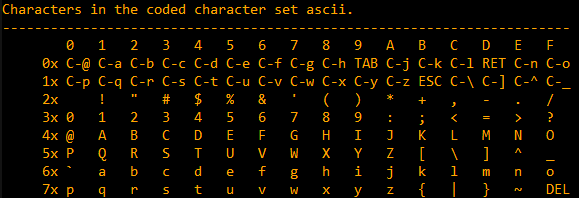
\includegraphics[width=0.8\textwidth]{ascii_clean.png}
\caption{Table \ac{ASCII} 7-bit dans Emacs}
\end{figure}

\dots avec la seule exception du caractère 0x7F.

Par exemple, \emph{chiffrons} les caractères de l'intervalle A-Z:

\begin{lstlisting}
#!/usr/bin/python

msg="@ABCDEFGHIJKLMNO"

print "".join(map(lambda x: chr(ord(x)^3), msg))
\end{lstlisting}

Résultat: \verb|CBA@GFEDKJIHONML|.

C'est comme si les caractères ``@'' et ``C'' avaient été échangés, ainsi que ``B''
et ``a''.

Encore une fois, ceci est un exemple intéressant de l'exploitation des propriétés
de XOR plutôt qu'un chiffrement:
le même effet de \emph{préservation de l'imprimabilité} peut être obtenu en échangeant
chacun des 4 bits de poids faible, avec n'importe quelle combinaison.

